% Standalone fragment; insert after verification_method.tex, before synthesis chapter.
% Historical 169f RTL snapshot and then-current testbenches. Do not relabel as compact reruns or STA.
\clearpage
\section{旧版修复基线：21 项逐项图证}
\label{sec:historical-21-evidence}
本节四幅图保留旧版修复基线的 21 项 testbench 结果，来源为仓库 \code{docs/evidence/20260930/final_rtl/}。
该轮 RTL 内容集合摘要前缀为 \code{169f957dc7fe}，不同于最新精简权重存储版本的 \code{fd885e882ad5}；两者都是内容摘要，不是 Git 提交号。
程序核对该轮成功状态、退出码、完成标记，以及全部日志和对应测试台的冻结 SHA。
后续归约测试台增加独立 scalar oracle 并完成双版本复验；最新 compact 三档结构顶层也已另立清单。
这两项补充见前述方法分析及本节末尾，不能把旧图中的日志替换成“最新 21 项已重跑”的声明。
每项列出计数、参考计算或断言对象及覆盖边界。\textbf{样本、输入码、断言、节拍和参数条件分别保留单位，不合成“总覆盖量”。}

\begin{figure}[H]\centering
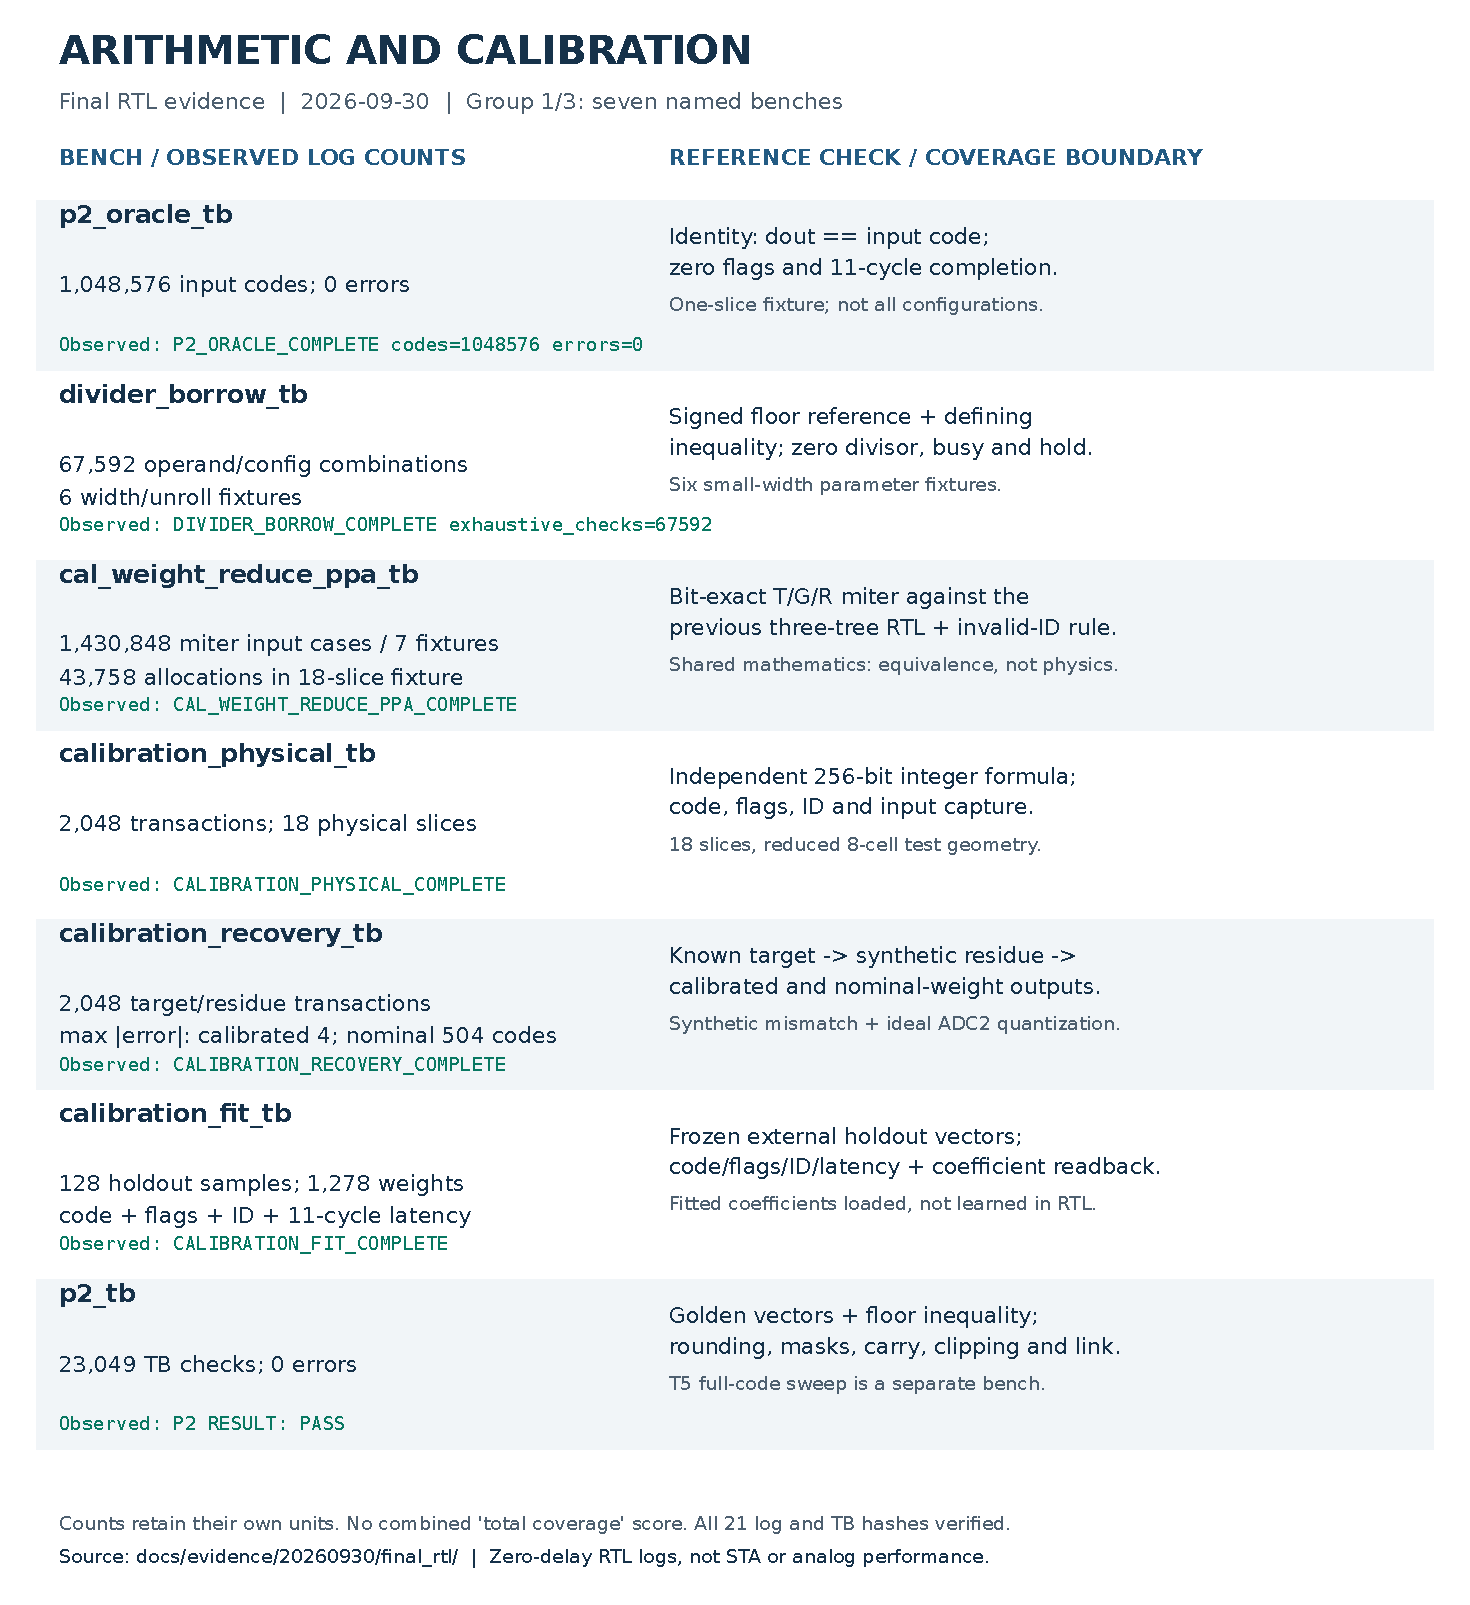
\includegraphics[width=.96\textwidth]{figures/final_regression_arithmetic.pdf}
\caption{旧版修复基线中算术与校准的七项回归。全码恒等测试只遍历一个简化配置；除法穷举覆盖六个小位宽参数实例；归约测试当时只判定新旧结构逐位一致，不能排除双方共同错误。独立 scalar 判据及双版本通过见图\ref{fig:reducer-scheduler-evidence}。物理权重、恢复和外部拟合测试分别使用独立宽整数公式、合成余差及冻结留出数据，不能相互替代。}
\label{fig:final-regression-arithmetic}
\end{figure}

\clearpage
\subsection{事务、取消与结构调度}
图\ref{fig:final-regression-protocol}取自旧版 21 项运行，其中 438 是结构顶层输出数，7,680 是该测试的检查节拍数，438 次延迟检查逐笔对应这些输出；三者不能相加为独立样本。
\code{review_recon_protocol_tb} 只打印完成标记，没有总检查计数，因此图中如实标为未记录。
\code{review_top_protocol_tb} 的 38 是测试台打印的固定输出数，图中不把它提升为独立的动态计数器证据。

\begin{figure}[H]\centering
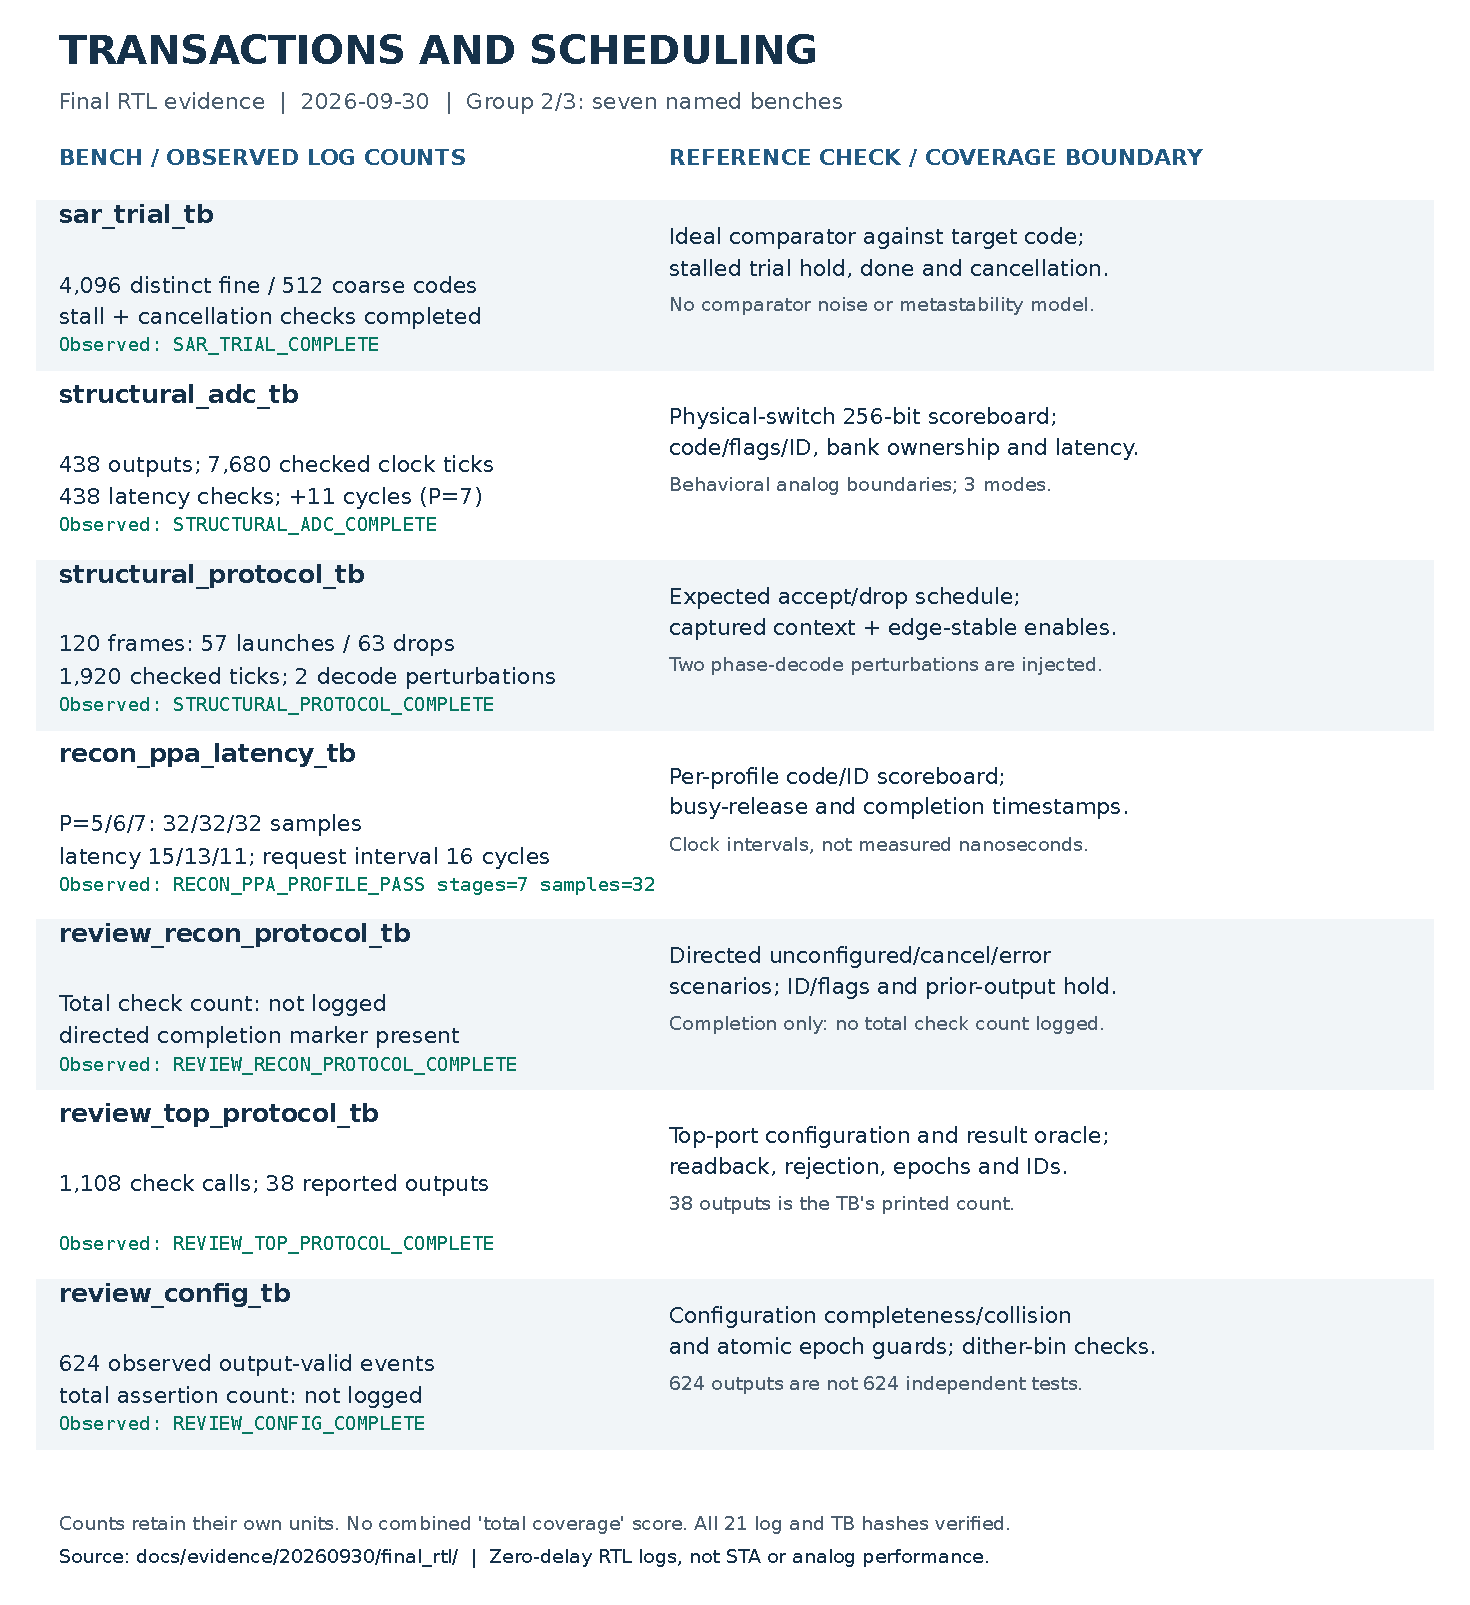
\includegraphics[width=\textwidth]{figures/final_regression_protocol.pdf}
\caption{旧版修复基线中事务和调度的七项证据。检查对象包括 SAR 停顿/取消、前后样本上下文隔离、ID/flags 对齐、无效配置屏蔽及 clear 后禁止旧 epoch 泄漏。展开级数 5/6/7 的输出延迟分别为 15/13/11 个完整时钟间隔，每项各 32 笔请求，属于旧版连续启动夹具；最新 compact 的 438 笔逐档回归另列。这些是功能仿真的拍数，不是门级纳秒时延或 640\,MHz 签核。}
\label{fig:final-regression-protocol}
\end{figure}

\clearpage
\subsection{基础模块、配置和兼容顶层}
图\ref{fig:final-regression-system}保留所有旧测试的原始计数器含义。
例如外设测试依次打印的各小计是累计值，不能再次相加；dither 的七种幅度/种子条件分别在 200,000 个观测周期内接收 196,866 或 200,000 笔有效输出。
\code{tree_mapping_tb} 在此目录中是 Verilator RTL 回归；实际综合后单元检查须引用另存的 Vivado/XSim 证据。

\begin{figure}[H]\centering
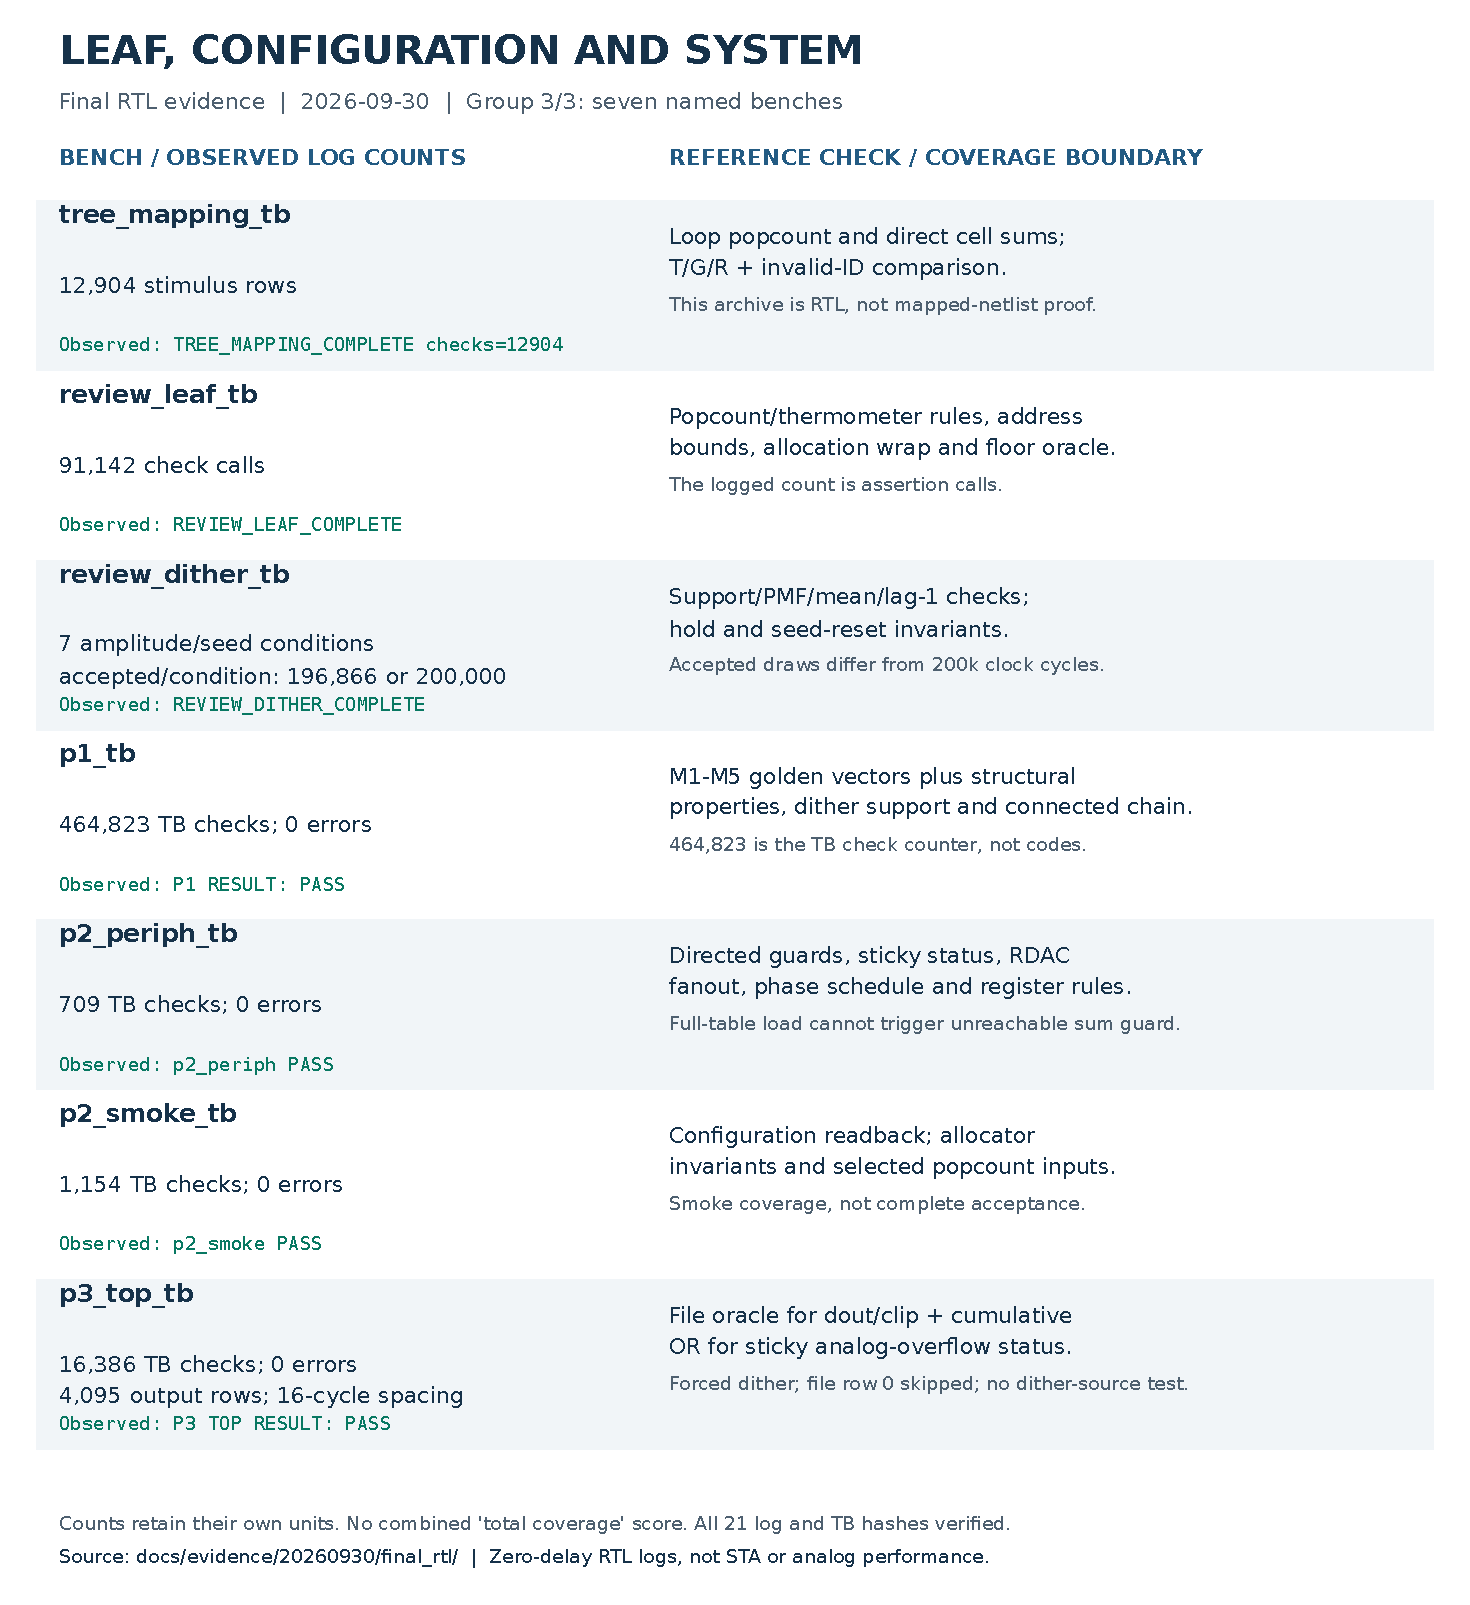
\includegraphics[width=\textwidth]{figures/final_regression_system.pdf}
\caption{旧版修复基线中基础模块、配置与兼容顶层的七项证据。兼容顶层比较 4,095 行输出，跳过向量文件第 0 行，并通过 force 注入 dither；因此不覆盖该模式下片内 dither 源。其 analog-overflow 按累积 OR 的粘滞口径比较，不能改用逐样本标志判断失配。}
\label{fig:final-regression-system}
\end{figure}

\clearpage
\subsection{日志中真正保留下来的定量观测}
图\ref{fig:final-regression-quantitative}只对存在的数据作图。
A、B 面板读取 \code{calibration_fit_tb.run.log} 的全部 128 条 \code{FIT_ROW}：逐样本实际码与期望码相同，flags 和 ID 无失配，延迟均为 11 拍；横轴是留出样本序号，不能称为模拟瞬态时间。
C 面板来自恢复测试的两个\emph{最大绝对误差}：标称权重为 504 码、校正权重为 4 码。日志没有逐样本误差分布，因此不能由两根柱子推导 RMS、SNDR 或 ENOB。

\begin{figure}[H]\centering
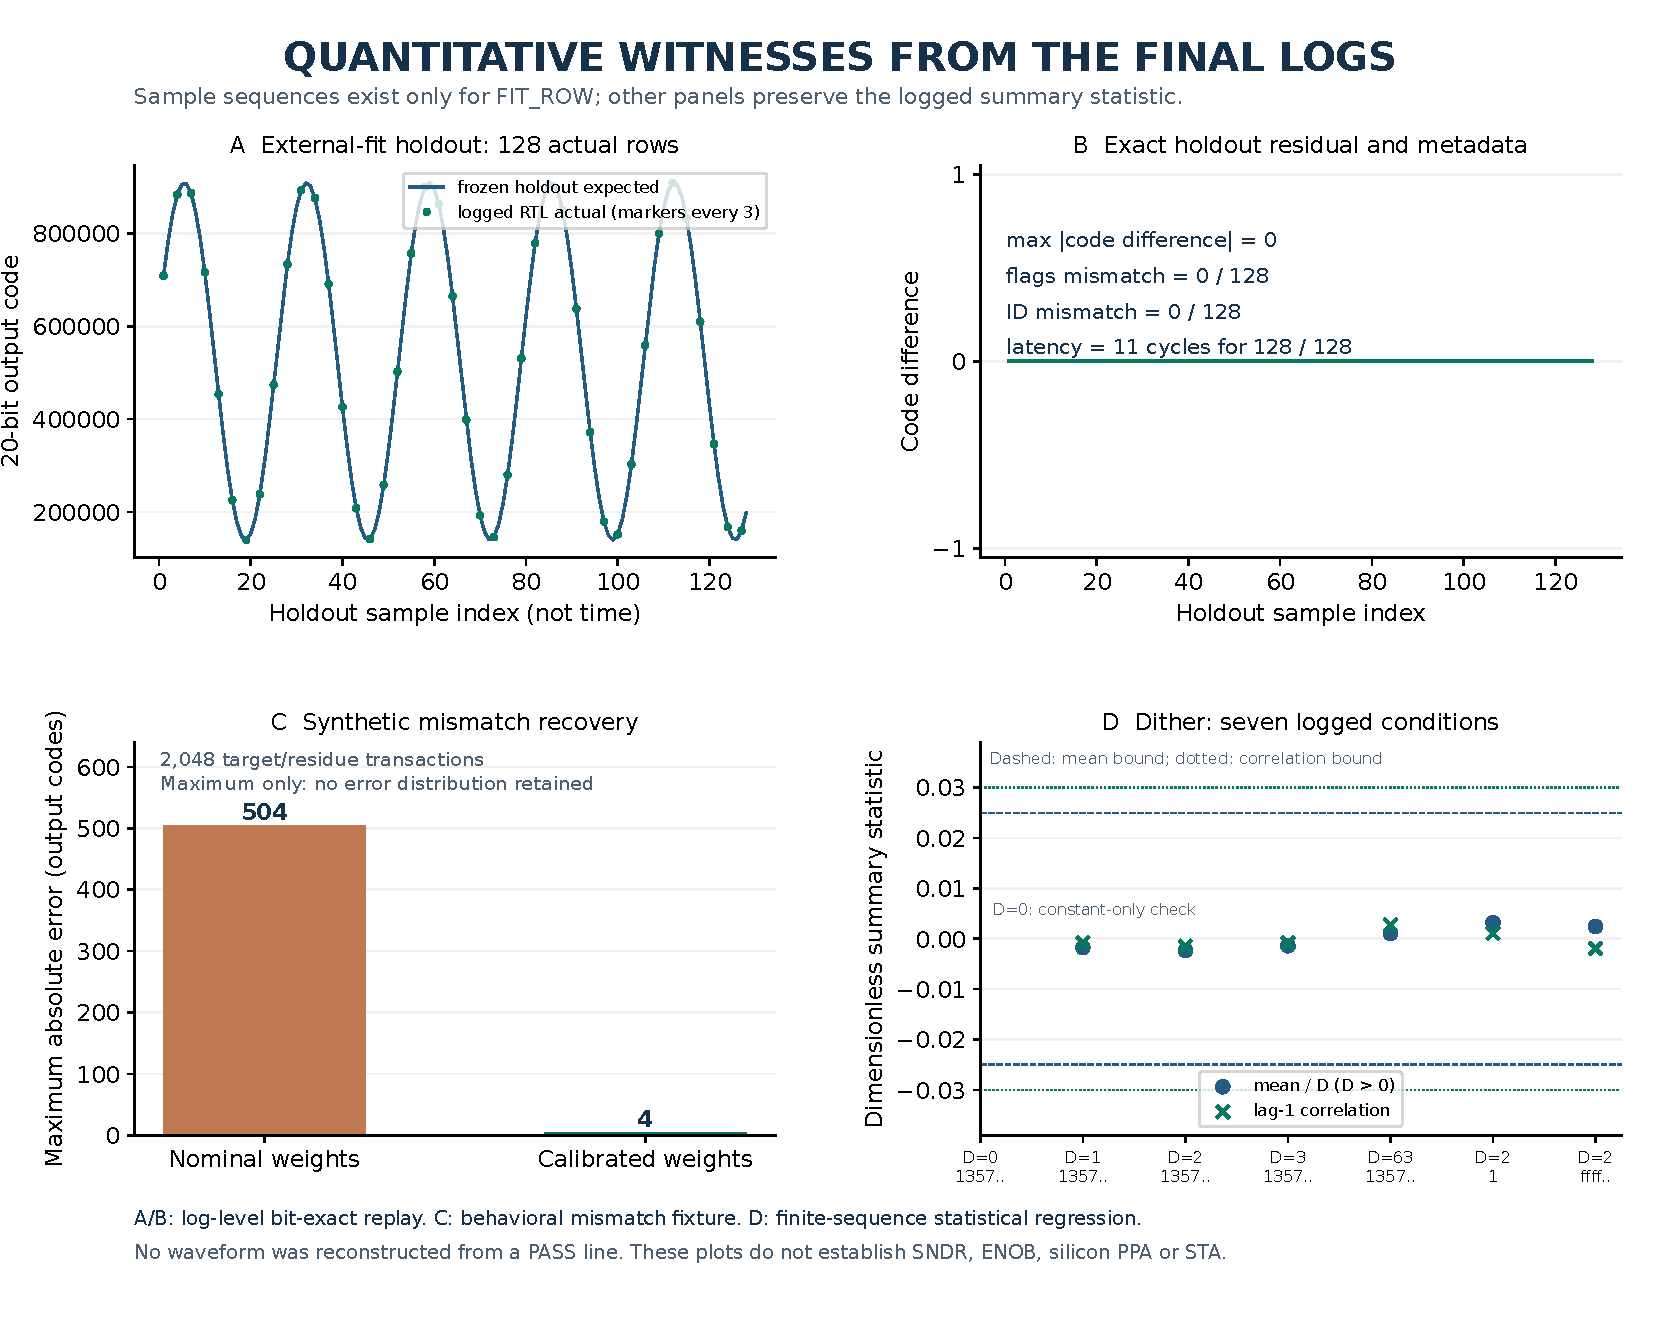
\includegraphics[width=\textwidth]{figures/final_regression_quantitative.pdf}
\caption{旧版修复基线日志的定量观测。A/B 为逐样本序列；C 为 2,048 笔合成失配测试的最大误差摘要；D 为七种 dither 条件的已打印统计量，均值除以幅度 $D$，虚线与点线分别为测试台的 $\pm0.025$ 与 $\pm0.03$ 门限。$D=0$ 方差为零，测试台跳过相关性计算，图中亦不将打印的初始化零值画成有效相关系数。}
\label{fig:final-regression-quantitative}
\end{figure}

D 面板还保留两项限制：日志只给六位小数的均值/相关系数，图不声称更高精度；PMF 检查虽由测试台执行，但该日志未保留各直方图 bin，故不能从完成标记补画分布。其余三个矩阵没有时序序列，使用证据矩阵而非合成波形。

制图脚本为 \code{audit_figures/make_final_regression_evidence.py}，在报告目录运行即可重建四张 PNG/PDF；每张同名 \code{audit_figures/final_regression_*.sha256.json} 记录输入日志、测试台、结果清单、脚本和图件的 SHA-256，并保存解析后的计数和绘图数据。源码来源清单 SHA-256 为 \code{8c781172b9b9db072462da9305f98ec2580099da5d4577b206274ae533327caa}。
本节四幅图只重建上述历史日志，不提供 STA、模拟电路或硅片性能签核。

\subsection{后续修复如何补充而不覆盖历史证据}
最新 compact 版本只改变合法系数写入时的恒零高位表达，生产源文件集合共 26 项，
完整摘要登记于 \code{docs/evidence/20260930/compact_profiles/rtl_compact_identity.json}。
同目录 \code{manifest.json} 及三份运行日志证明：P5/P6/P7 分别编译、运行退出 0，
各包含 3 种模式、18 个物理 slice、438 次输出、438 次延迟检查和 7,680 个协议检查节拍，
精确重构延迟分别为 15、13、11 拍。
图件 \code{figures/31_divider_profiles.png} 已按这些新日志重建，
其输入摘要见 \code{audit_figures/31_source_hashes.json}。
此次未重新运行旧 21 项的全部 testbench，亦未重跑旧版 32 笔连续启动夹具，
因此这里不以三档通过替代一次未执行的全量回归。

归约器在两个工具版本上的完整复验及共同错误负控，见图\ref{fig:reducer-scheduler-evidence}。
其生产模块未因测试台调度修复而改变，且摘要与 compact 源码一致；
该图的制图脚本与来源清单分别为 \code{audit_figures/make_reducer_scheduler.py} 和
\code{audit_figures/39_source_hashes.json}。
Python 镜像的 55,432 个小几何输入对与 918 项非 slow 回归也在前述小节独立说明，
不混入此处 21 项 RTL 图证的计数。
